\section{Methodology}

\begin{figure}
    \centering
    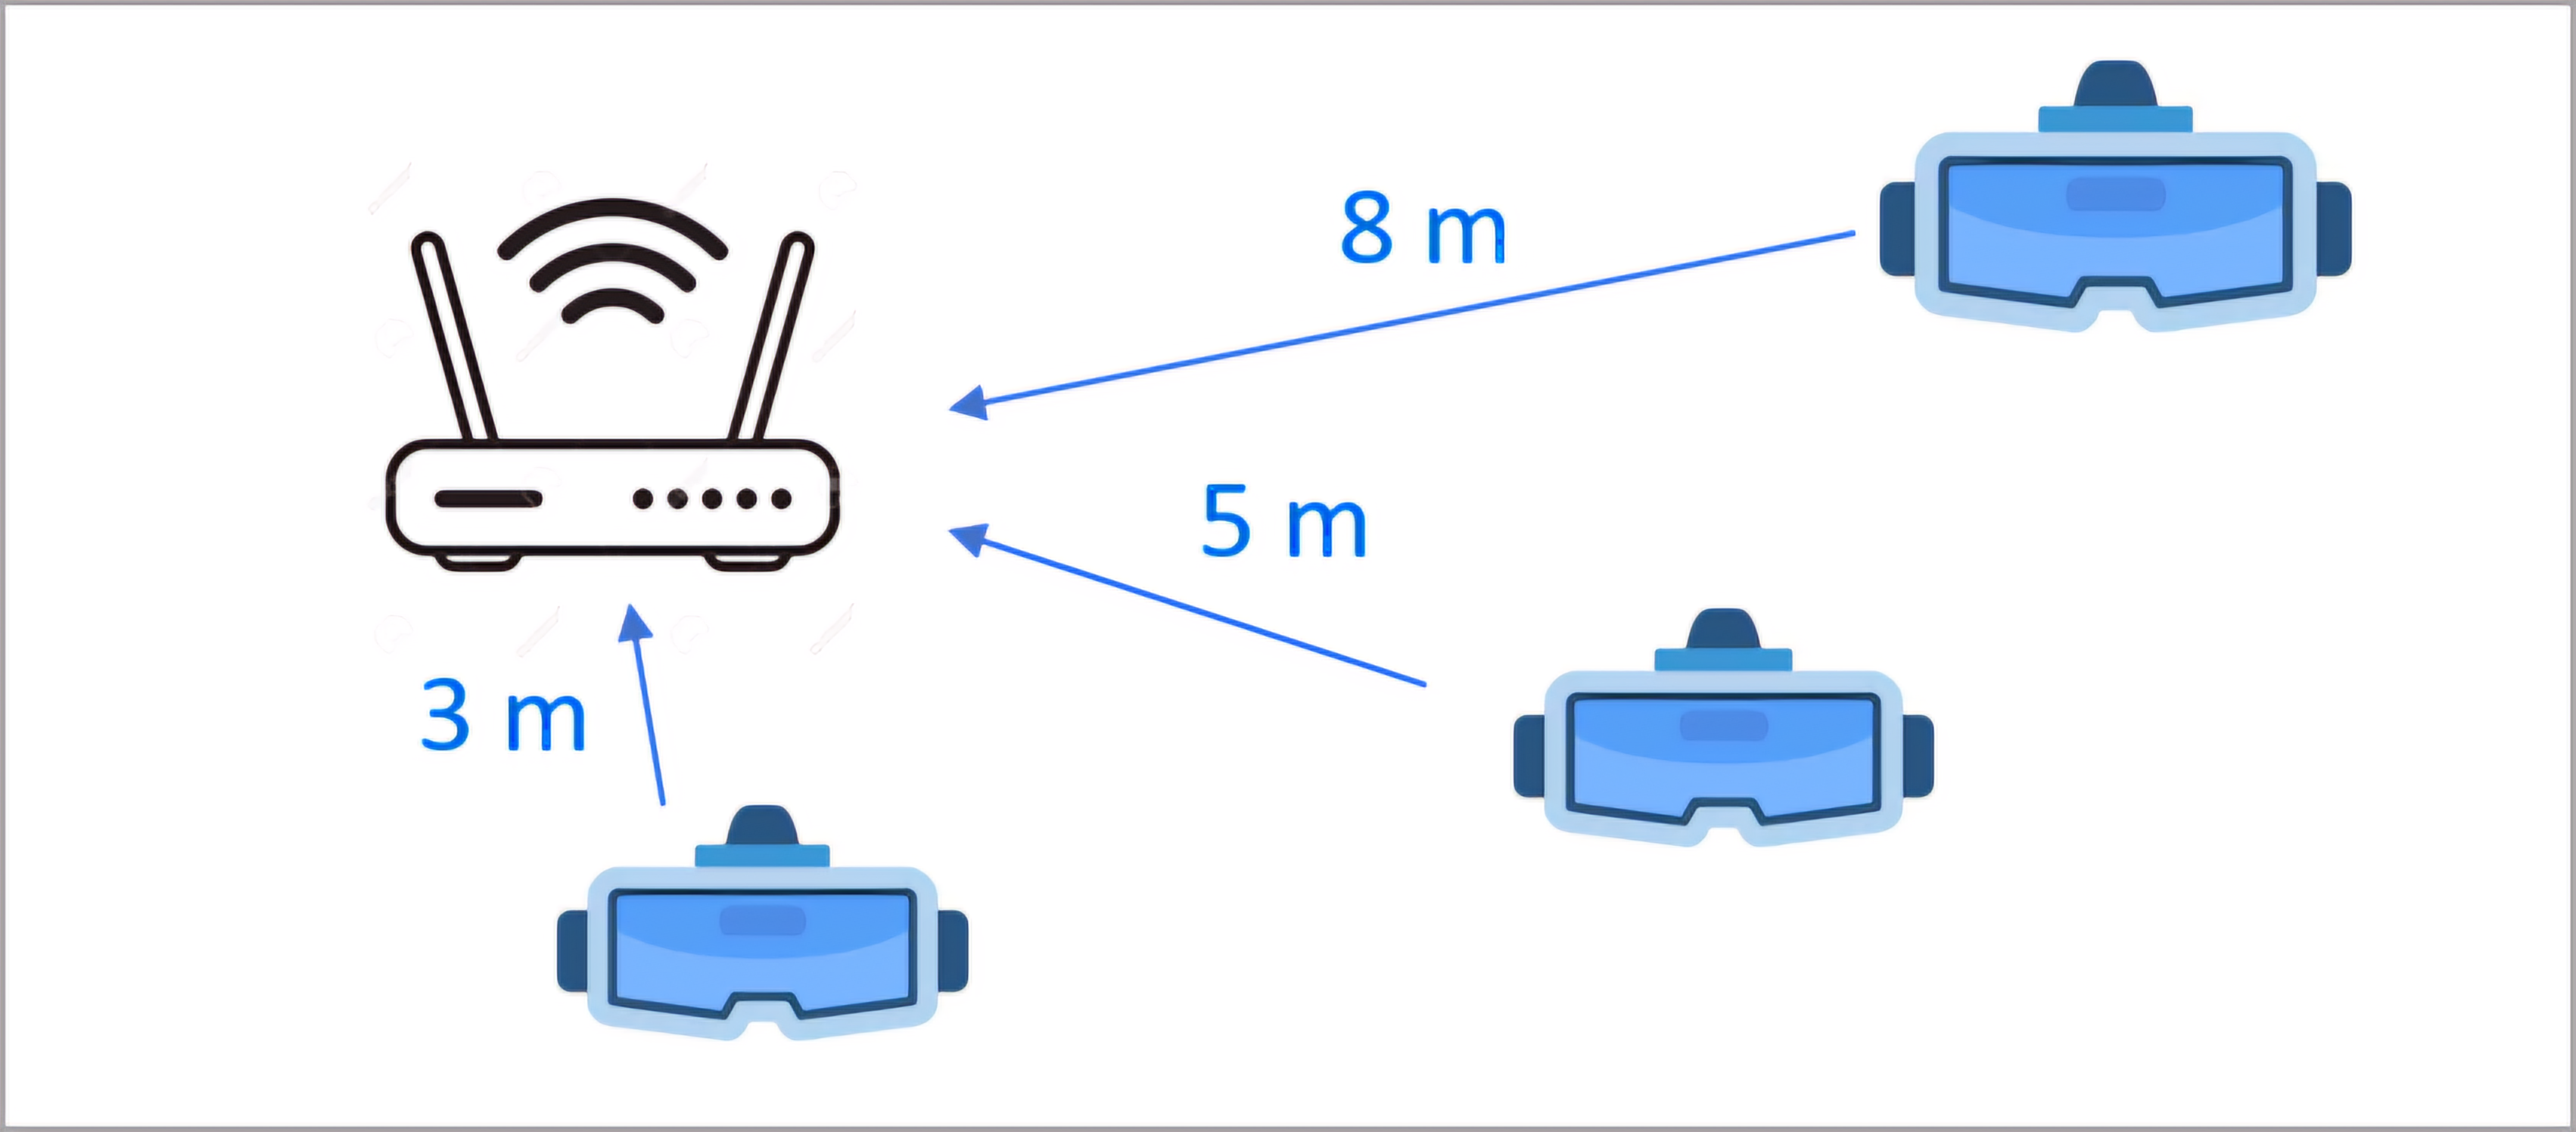
\includegraphics[width=0.48\textwidth, height=4.8cm]{figures/3_5_8_scenario.png}
    \caption{XR Scenario}
    \label{fig:xr}
\end{figure}
% \begin{figure}
%     \centering
%     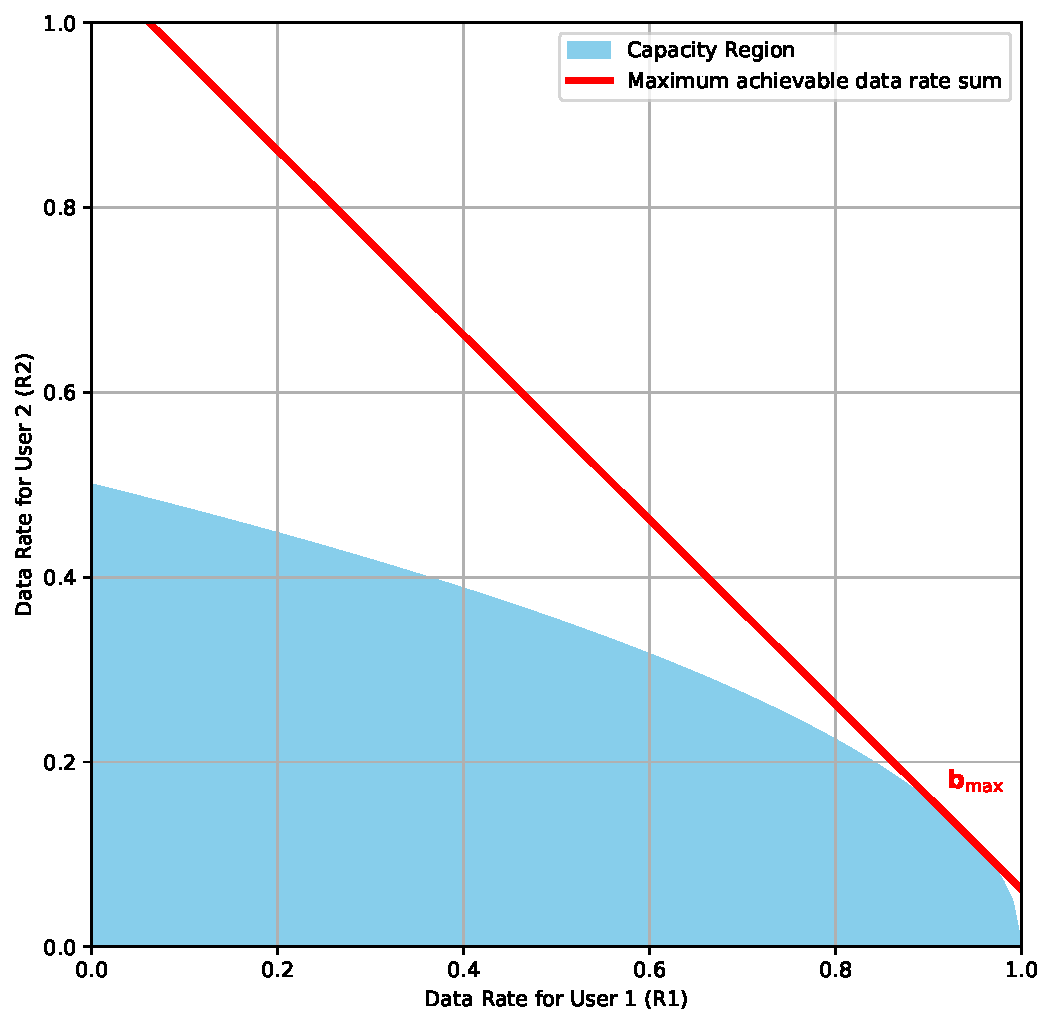
\includegraphics[width=6cm]{figures/Capacity_Region.pdf}
%     \caption{Capacity Region for two Users}
%     \label{fig:capacity_region}
% \end{figure}

% Repeat problem explanation
% Copy formulation from slides for energy minimization problem: explain and break it down into simpler subproblem by defining b, for example
% Explain GDFE from Chapter 5
% Explain minPMAC logic, ellipsoid, provide code from book , explain the concept of time sharing or vertex sharing
The Generalized Decision-Feedback Equalizer (GDFE) resolves multiuser crosstalk issues. To achieve this, each user's data is detected based on all previously decoded users with each symbol \cite{book}, \cite{yu2004sum}. % By assuming that the channel is non-singular, and we are using ideal code {\color{red} (Gap = 0)}, 

This work compares the performance of non-linear (GDFE) receivers \cite{GDFE} and linear receivers\cite{chang1966synthesis}, both using basic OFDM.  The specific focus is energy consumption. Initially, the receiver analysis uses the Simultaneous Water-Filling (SWF) algorithm\cite{book} with the linear receiver.  This SWF optimizes the sum data rate for a given available energy. Subsequently, a receiver uses the GDFE, targeting the data rate determined by the SWF algorithm, to minimize energy. The objective is to demonstrate how the GDFE receiver can substantially reduce energy consumption in attaining the same SWF data rate values obtained. 
% {\color{red} why GDFE results in a better energy preservation?}

Notation includes: $U$ denotes the number of users. $\bar{N}$ represents the number of tones. $L_x$ and $L_y$ are the total number of users' antennas and the total number of antennas at the access point, respectively. $L_{x,u}$ is the number of antennas for the $u^{th}$ user. Moreover, the subscripts $u$ and $n$ represent user $u$ and $n^{th}$ tone, respectively. For instance, $H_u$ is user $u$'s channel matrix. 
% The duality between these two problems arises from their shared Lagrangian frameworks. Both problems involve a common Lagrangian term in their expressions, which indicates a zero duality gap for their respective optimizations under certain conditions. The Lagrangian expressions for both problems differ in how the parameters $\theta$ and $w$ are interpreted (as either given constants or Lagrange multipliers) and in the terms related to incremental change constraints.
There are two weighted-sum optimization problems: Energy Sum Minimization (\ref{Esum}) and Data Rate Sum Maximization (\ref{Rsum}).
\subsection{Energy Sum Minimization} \label{Esum}
The weighted Energy Sum Minimization is formulated as follows:
\begin{equation}
\begin{aligned}
\min_{\left\{R_{\boldsymbol{xx}}{(u)} \right\}} \quad & \sum_{u=1}^U w_u \cdot \operatorname{trace} \underbrace{\{R_{ \boldsymbol{x} \boldsymbol{x}}{(u)}\}}_{\mathcal{E}_u}\\
\textrm{s.t.} \quad & \mathbf{b} \succeq \left[b_{1, \min }, b_{2, \min }, \ldots, b_{U, \min }\right]^*\\
  &\mathcal{E}\geq0    \\
\end{aligned}
\end{equation}
Where $R_{\boldsymbol{xx}}(u)$ and $b_{u,\operatorname{min}}$ are the autocorrelation matrix and user $u$'s minimum data rate, respectively. Also, the vector $w \in \mathbb{R}_{0+}^U$ represents non-negative weights for each user's energy.
The corresponding Lagrangian function is:
% \begin{equation}
% \begin{aligned}
% \mathcal{L}\left(R_{\boldsymbol{x} \boldsymbol{x}}(n), \boldsymbol{b}, \boldsymbol{w}, \boldsymbol{\theta}\right)=\sum_{u=1}^U(&w_u \cdot\left[\sum_{n=0}^{\bar{N}} \operatorname{trace}\left\{R_{\boldsymbol{x} \boldsymbol{x}}(u, n)\right\}\right]+\\
% &\theta_u \cdot\left\{\left[\sum_{n=0}^{\bar{N}-1} b_{u, n}\right]-b_u\right\})
% \end{aligned}
% \end{equation}
\begin{equation}
\begin{aligned}
\mathcal{L}_{\min E}\left(R_{\boldsymbol{x} \boldsymbol{x}}, \boldsymbol{b}, \boldsymbol{w}, \boldsymbol{\theta}\right)=\max _{\boldsymbol{\theta}} \min _{R_{\boldsymbol{x} \boldsymbol{x}}} &\sum_{u=1}^U  w_u \cdot \operatorname{trace}\left\{R_{\boldsymbol{x} \boldsymbol{x}}(u)\right\}\\ &+ \theta_u \cdot b_u-\theta_u \cdot b_{\min , u}
\end{aligned}
\end{equation}
\subsection{Data Rate Sum Maximization} \label{Rsum}
The weighted Data Rate Sum Maximization problem can be formulated as follows:
\begin{equation}
\begin{aligned}
\max _{\left\{R_{\boldsymbol{x} \boldsymbol{x}}{(u)}\right\}} \quad &\sum_{u=1}^U \theta_u \cdot b_u \\
\textrm{s.t.} \quad &\mathcal{E}_{\boldsymbol{x}} \preceq\left[\mathcal{E}_{1,\max}, \mathcal{E}_{2,\text{max}},\ldots,\mathcal{E}_{U,\text{max}}\right]^*\\
& \mathbf{b} \succeq 0
\end{aligned}
\end{equation}
Similar to the previous part, we can expand the Lagrangian function:
\begin{equation}
\begin{aligned}
\mathcal{L}_{\max R}\left(R_{\boldsymbol{x} \boldsymbol{x}}, \boldsymbol{b}, \boldsymbol{w}, \boldsymbol{\theta}\right)=\min _{\boldsymbol{w}} \max _{R_{\boldsymbol{x} \boldsymbol{x}}} &\sum_{u=1}^U w_u \cdot \operatorname{trace}\left\{R_{\boldsymbol{x} \boldsymbol{x}}(u)\right\}\\ &+\:\theta_u \cdot b_u-w_u \cdot \mathcal{E}_{\max , u}
\end{aligned}
\end{equation} 

The common term $w_u \cdot \operatorname{trace}\left\{R_{\boldsymbol{x} \boldsymbol{x}}(u)\right\} + \theta_u \cdot b_u$ in both optimization problems implies their duality. Therefore, a primal-dual approach solves the optimization problem.This locates the optimal autocorrelation matrix $R_{\boldsymbol{xx}}$, while fulfilling both the data rate and energy constraints. 
% Both problems involve a common Lagrangian term in their expressions, which indicates a zero duality gap for their respective optimizations under certain conditions. The Lagrangian expressions for both problems differ in how the parameters $\theta$ and $w$ are interpreted (as either given constants or Lagrange multipliers) and in the terms related to incremental change constraints.


% As we can see, there is a common term in both optimization problems, and our algorithm tries to optimize these two problems simultaneously. Specifically, the algorithm locates the optimal $R_{\boldsymbol{xx}}$, while fulfilling both the data rate and energy constraints. 
It can be proven that the aforementioned optimization problems can be solved for each tone separately. In other words, an independent GDFE is assigned to each tone, and the total energy can be calculated by summing up all tones\cite{book}. The corresponding energy minimization problem for each tone is as follows:
\begin{equation} \label{tonalE}
    \begin{aligned}
        \min_{\left\{R_{\boldsymbol{x} \boldsymbol{x}}{(u, n)}\right\}} \quad &\sum_{u=1}^U \sum_{n=0}^{\bar{N}} w_u \cdot \operatorname{trace}\left\{R_{\boldsymbol{x} \boldsymbol{x}}(u, n)\right\} \\
        \textrm{s.t.} \quad &\mathbf{b}=\sum_{n=0}^{\bar{N}}\left[b_{1, n}, b_{2, n}, \ldots ,b_{U, n}\right]^* \succeq \boldsymbol{b}_{\min } \succeq \mathbf{0}
    \end{aligned}
\end{equation}
Where $R_{\boldsymbol{xx}}(u,n)\in\mathbb{R}^{L_{x,u}\times L_{x,u}}$ is the autocorrelation matrix of $\boldsymbol{x}$ for user $u$ on the $n^{th}$ tone. 

Similarly, the data rate maximization problem per each tone is:
\begin{equation}
\begin{aligned}
\max_{\left\{R_{\boldsymbol{x} \boldsymbol{x}}{(u, n)}\right\}} \quad &\sum_{u=1}^U \theta_u \cdot\left\{\sum_{n=0}^{\bar{N}} b_{u, n}\right\} \\
\textrm{s.t.} \quad &\mathcal{E}=\sum_{n=0}^{\bar{N}}\left[\mathcal{E}_{1, n}, \mathcal{E}_{2, n}, \ldots, \mathcal{E}_{U, n}\right]^* \preceq \boldsymbol{\mathcal{E}}_{\max } \;\;.
\end{aligned}
\end{equation}
Equation \ref{tonalE} 's Lagrangian function is:
\begin{equation} \label{minmaxE}
\begin{aligned}
\mathcal{L}_{\min E}\left(R_{\boldsymbol{x} \boldsymbol{x}}, \boldsymbol{b}, \boldsymbol{w}, \boldsymbol{\theta}\right)&=\left(\sum_{u=1}^U \theta_u \cdot b_u\right)
+ \\
& \hspace{-1.5cm} \sum_{n=0}^{\bar{N}-1}\{\underbrace{\sum_{u=1}^U\left[w_u \cdot \operatorname{trace}\left\{R_{\boldsymbol{x} \boldsymbol{x}}(u, n)\right\}-\theta_u \cdot b_{u, n}\right]}_{\mathcal{L}_n\left(R_{\boldsymbol{x} \boldsymbol{x}}(n), \boldsymbol{b}_n, \boldsymbol{w}, \boldsymbol{\theta}\right)}\}
\end{aligned}
\end{equation}
Where $R_{\boldsymbol{x} \boldsymbol{x}}(n)=\operatorname{blkdiag}\left\{R_{\boldsymbol{x} \boldsymbol{x}}(U, n), \ldots, R_{\boldsymbol{x} \boldsymbol{x}}(1, n)\right\}$, and the operator $\operatorname{blkdiag}$ aligns matrices along the diagonal of another matrix. The term $\mathcal{L}_n\left(R_{\boldsymbol{x} \boldsymbol{x}}(n), \boldsymbol{b}_n, \boldsymbol{w}, \boldsymbol{\theta}\right)$ is called the Tonal Lagrangian term. Since $\mathcal{L}_n$ does not depend on $b_u$, minimizing the tonal lagrangian term is synonymous with optimizing: 
\begin{equation}
\mathcal{L}_{\min E}(\boldsymbol{\theta}, n) \triangleq \min _{\left\{R_{\boldsymbol{xx}}(u, n), b_{u, n}\right\}} \mathcal{L}\left(R_{\boldsymbol{xx}}(n), \boldsymbol{b}_n, \boldsymbol{w}, \boldsymbol{\theta}\right)    
\end{equation}
Therefore, the min-max problem \ref{minmaxE} reduces to :
\begin{equation} \label{final}
\mathcal{L}_{\min E}^*=\max _{\boldsymbol{\theta}}\{\left[\sum_{n=0}^{\bar{N}-1} \mathcal{L}_{\min E}(\boldsymbol{\theta}, n)\right]+\hspace{-0.5cm}\underbrace{\sum_{u=1}^U \theta_u \cdot b_u}_{\text {independent of } R_{\boldsymbol{xx}}(u, n), n}\hspace{-0.5cm}\}
\end{equation}

Moreover, the data rates must lie in the system's capacity region. The capacity region, denoted as $\mathcal{C}(b)$, refers to the set of all possible rate vectors $b$ for users with independent messages, where each message employs a code that achieves the single-user capacity. This code is used for all systems and differences in their performance therefore solely derives from the GDFE improvement over the linear receiver.  This set characterizes the rates at which all users can be reliably decoded with a negligible average error probability by a Maximum A Posteriori (MAP) detector or equivalently, a Maximum Likelihood (ML) detector with equally likely messages for all independent users. The capacity region is essentially the combination of rates at which the system can operate such that all users' messages are delivered correctly. %Figure \ref{fig:capacity_region} depicts the capacity region for two users. 
The capacity region follows from the Shannon capacity formula as \cite{shannon}: 
\begin{equation}
0 \leq b_n %\sum_{\boldsymbol{u} \subseteq \boldsymbol{U}} b_{u, n}
\leq \log _2\left|\left(\sum_{u=1}^U \widetilde{H}_{u, n} \cdot R_{\boldsymbol{x} \boldsymbol{x}}(u, n) \cdot \widetilde{H}_{u, n}^*\right)+I\right|
\end{equation}

$\tilde{H}_{u, n}=R_{N N}^{-1 / 2}(n) \cdot H_{u, n}$ is the equivalent-white-noise channel per each tone.
% A multiple-input-multiple-output (MIMO) system with additive white Gaussian noise (AWGN) can be described as
% \begin{equation}
% \boldsymbol{y}=H \cdot \boldsymbol{x}+\boldsymbol{n}
% \end{equation}

% Where $H \in \mathbb{R}^{L_y \times L_x}$ is the channel matrix, and $x$, $y$ are the transmitted and received signals respectively. 
A semi-definite programming (SDP) method solves the inner part of the optimization problem \ref{final} ($\mathcal{L}_{\min E}(\boldsymbol{\theta}, n)$), while an Ellipsoid method \cite{yudin1976constrained} 
% {\color{red} Correct the citation part} optimizes the outer part. 

If the channel matrix $H_{u,n}$ is non-singular with the ideal common codes mentioned ($\Gamma = 0 \textrm{dB}$), the ellipsoid method finds a unique optimal solution. In other words, the system assigns different dimensions, such as time and frequency, to each user separately. However, if the channel is singular, the Hessian matrix computed at each ellipsoid-method iteration degradeds, and the optimization problem does not have a unique solution. In this case, the algorithm allows more than one user to use some specific dimensions at the same time, which is known as “time-sharing”. When the users “time-share” with one another, the algorithm only finds the weighted sum.  A separate time-sharing step then applies to ensure all users meet their target data rate.  

% If the optimal point of energy lies inside the capacity-energy region, the Ellipsoid algorithm can find this point successfully. However, as we get closer to the boundary of the capacity region, the Hessian matrix constructed in the Ellipsoid algorithm will become singular (the minimum eigenvalue of the Hessian matrix will get closer to zero). Under these conditions, the system is stressed, making it more challenging for the Ellipsoid method to converge.

% {\color{red}this paragraph or above} Our algorithm is capable of stressing the system as much as possible so that each user doesn't experience low data rate. However, this goal is within reach only by using time-sharing, which is synonymous with allowing users to use the same amount of resources at the same time.

This minPMAC algorithm appears as Algorithm 2.  Initially, the SWF algorithm provides first ellipsoid parameters. Then, minPMAC alternates between two optimization problems until convergence. It prioritizes the users' decoding process based on $\theta$ at each iteration.

% \begin{table}[t]
%     \caption{Notation Explanation}
%     \centering
%     \begin{tabular}{|c|c|}
%     \hline
%        \textbf{Parameter}  &  \textbf{Explanation}\\ \hline
%        $U$ & Number of users\\ 
%        $N$ & Number of tones\\
%        $L_x$ & Total number of users' antennas\\
%        $L_y$ & Total number of antennas at the access point\\ 
%        $L_{x,u}$ & user $u^{th}$ number of  antennas \\  \hline
        
%     \end{tabular}
%     \label{tab:ranging-imu-params}
% \end{table}



\begin{algorithm}[t]
	\caption{SWF} 
    \State \textbf{Inputs:} $H, L_x, R_{nn}$
		\For {$u=1,2,\ldots,U$}
            \State $R_{\text {noise}}(u) \triangleq \sum_{i \neq u} H_i \cdot R_{\boldsymbol{x} \boldsymbol{x}}(i) \cdot H_i^*+R_{\boldsymbol{nn}}$
            \vspace{0.1cm}\State $R_{\text {noise }}^{-1 / 2}(u) \cdot H_u=F_u \cdot \Lambda_u \cdot M_u^*$
            \vspace{0.1cm}\For{$\ell = 1,2,\ldots, L_x$}
                \State $\mathcal{E}_{u,\ell} = \operatorname{max} \left\{0, {\frac{1}{L_x}}\left(\mathcal{E}_u - \sum_{k=1}^{L_x}\frac{1}{\lambda_{u,k}^2}\right) - \frac{1}{\lambda_{u,\ell}^2}\right\}$
            \vspace{0.1cm}
            \EndFor
		\EndFor
\State \textbf{return} $\mathcal{E}_u$
\end{algorithm}







% \vspace{30 pt}

\begin{algorithm}[t]
	\caption{minPMAC} 
	% \begin{algorithmic}[1]
    \State \textbf{Inputs:} $H$, $L_{xu}$, $b_u$, $w$ 
    \vspace{0.1cm}
    \State \textbf{Initialize:} $A$, $\theta$ using SWF
    % \vspace{0.1cm}
    % \State $Idx_{END} = \operatorname{cumsum}(L_{xu})$
    % \vspace{0.1cm}
    % \State $Idx_{START} = [1, Idx_{END}(1:end-1)+1]$ 
    % \vspace{0.1cm}
    % \State $D \in \mathbb{R}^{U\times U}, \quad D_{i,i} = 1, D_{i,i+1} = -1 \quad \forall 1\leq i \leq U-1$
    % \vspace{0.1cm}
    \While {the sum rate doesn't converge}
    \vspace{0.1cm}
    \State $\pi \triangleq$ Indices of sorted $\theta$ in descending order
    \vspace{0.1cm}
       \For {$n = 1,2, \ldots,\bar{N}$}
        \vspace{0.1cm}
            \For{$u = 1,2,\ldots,U$}
                \vspace{0.1cm}
                \State \hspace{-0.3cm} $\footnotesize \mathcal{E}_{u,n} = \operatorname{trace}\left(R_{\boldsymbol{x} \boldsymbol{x}}\left(\pi^{-1}(u), n\right)\right)$
                \vspace{0.1cm}
                \State \hspace{-0.3cm} $\footnotesize \mathcal{R}_{u,n} \triangleq  \log _2\left|\sum_{i=u}^U \tilde{H}_{\pi^{-1}(i), n} \cdot R_{\boldsymbol{x} \boldsymbol{x}}\left(\pi^{-1}(i), n\right) \cdot \tilde{H}_{\pi^{-1}(i), n}^*+I\right|$
            \EndFor 
            \vspace{-0.7cm}
            \State \begin{equation*}
            \hspace{0.5cm} b_{u,n}^*=\underset{{R_{\boldsymbol{xx}}}}{\operatorname{argmin}} \quad \sum_{u=1}^U w_{u} \cdot \: \mathcal{E}_{u,n}- \left(\theta_{\pi^{-1}(u)}-\theta_{\pi^{-1}(u+1)}\right) \cdot \: \mathcal{R}_{u,n} \end{equation*}
            \vspace{-0.6cm}
            \State \begin{equation*}
                \hspace{-2cm} \textrm{s.t.} \quad R_{\boldsymbol{xx}}  \succeq \mathbf{0}
            \end{equation*}
    \EndFor 
    \vspace{0.1cm}
    \State $g = \sum_{n = 1}^{\bar{N}}  b_{u,n}^* - b_u$
    \vspace{0.1cm}
	\State $\tilde{g} = \frac{1}{\sqrt[]{g^TAg}}g$
    \vspace{0.1cm}
    \State $\theta = \theta - \frac{1}{U+1}\frac{Ag}{\sqrt[]{g^TAg}}$
    \vspace{0.1cm}
    \State $A = \frac{U^2}{U^2-1}(A - \frac{2}{U+1} A \tilde{g}\tilde{g}^T A)$
    % \vspace{0.1cm}
    % \State $\mathcal{S} = \left\{i \: | \: \theta_i < 0\right\}$
    % \vspace{0.1cm}
    % \While {$\mathcal{S} \neq \left\{\right\}$}
    %     \State $g = \mathbf{0}$
    %     \vspace{0.1cm}
    %     \State $g(\mathcal{S}(1)) = 1$
    %     \vspace{0.1cm}
    % 	\State $\tilde{g} = \frac{1}{\sqrt[]{g^TAg}}g$
    %     \vspace{0.1cm}
    %     \State $\theta = \theta - \frac{1}{U+1}\frac{Ag}{\sqrt[]{g^TAg}}$
    %     \vspace{0.1cm}
    %     \State $A = \frac{U^2}{U^2-1}(A - \frac{2}{U+1} A \tilde{g}\tilde{g}^T A)$
    %     \vspace{0.1cm}
    %     \State $\mathcal{S} = \left\{i \: | \: \theta_i < 0\right\}$
    % \ENDWHILE
\ENDWHILE
\vspace{0.1cm}
\State \textbf{return} $b_{u,n}^*, \: \mathcal{E}_{u,n}$
\end{algorithm}
